\selectlanguage{english}
\settitle{Protecting SSH authentication with TPM 2.0}
\setauthor[N.~Iooss]{Nicolas Iooss\\
\email{nicolas.iooss@ledger.fr}}
\institute{\raisebox{-0.2cm}{
\includegraphics[width=0.6cm]{ProtectingSshAuthenticationWithTpm20/img/donjon-black.pdf}} Ledger Donjon}

\setcounter{tocdepth}{2}  % show sections and subsections in PDF index

\ifdefined\pdftrailerid
  \pdftrailerid{} % For reproducible build
\fi

\maketitle
\index{Iooss, N.}

\begin{abstract}

For quite some time, desktop computers have been embedding a security chip.
This chip, named Trusted Platform Module (TPM), provides many features including the ability to protect private keys used in public-key cryptography.
Such keys can be used to authenticate users in network protocols such as Secure Shell (SSH).

Software stacks which enable using a TPM to secure the keys used in SSH have been available for several years.
Yet their use for practical purposes is often documented only from a high-level perspective, which does not help answering questions such as: can the security properties of keys protected by a TPM be directly applied to SSH keys?

This is a non-trivial question as for example those properties do not apply for disk encryption with sealed keys.
Therefore this article fills the documentation gap between the TPM specifications and the high-level documentations about using a TPM to use SSH keys.
It does so by studying how SSH keys are stored when using \texttt{tpm2-pkcs11} library on a Linux system.

\end{abstract}

\section{Introduction}

\subsection{SSH, TPM and how they can be used together}

When using remote services, users need to be authenticated. Every
protocol relies on different mechanisms to implement user
authentication: a secret password, an RSA key pair on a smartcard, a
shared secret used with a TOTP (Time-based One-Time Password)
application on a smartphone, etc. Many authentication mechanisms are
considered highly secure nowadays (for example the ones relying on
dedicated devices such as smartcards). However when discussing habits
with other people, it seems that many still continue to use very weak
mechanisms instead, even for protocols such as SSH which can be
considered as mainly used by people interested in computer science
(developers, system administrators, researchers, etc.).

SSH (Secure Shell) is a network protocol which can be used to access a
remote command-line interface (``a shell''), transmit files to a server,
forward other network protocols, etc. It is possible to use public-key
cryptography to authenticate to an SSH server, with an unencrypted
private key. Such a configuration can be reproduced by running
\texttt{ssh-keygen -t rsa -N ""} on the client. Doing
so, a client RSA private key is generated in
\texttt{.ssh/id\_rsa} and its matching public key is
saved in \texttt{.ssh/id\_rsa.pub} (in the home
directory of the user who ran this command). By copying the content of
\texttt{.ssh/id\_rsa.pub} into the list of their
authorized keys on an SSH server (for example in remote file
\texttt{.ssh/authorized\_keys})\footnote{The copy of
  the public key to \texttt{.ssh/authorized\_keys} can
  be done using a tool such as \texttt{ssh-copy-id}
  (\url{https://manpages.debian.org/stretch/openssh-client/ssh-copy-id.1.en.html}).},
the user can establish connections to the SSH server without entering
any password. However, if someone gets access to the content of
\texttt{.ssh/id\_rsa} (for example by executing
malicious software on the victim's computer or by getting the hard drive
while the computer is powered down), this attacker can impersonate the
victim and connect to the SSH server independently of the victim.

In order to prevent this attack, it is recommended to protect the
private key with a secret password. Doing so prevents an attacker from
getting the key by directly copying the file, but this does not prevent
malicious software from stealing the private key. Indeed, such software
can record the keystrokes in order to steal the password, or dump the
memory of the SSH agent process while the private key is loaded.

To increase the protection of the private key even more, it is
recommended to use dedicated hardware to store it. Several manufacturers
have been building such hardware for more than ten years and nowadays
users can buy (in alphabetical order) a Ledger Nano, a Nitrokey, a PGP
smartcard, a Solo security key, a Titan security key, a Yubikey, or one
out of many other products. All these products work in a similar way:
they store a private key and they enable users to authenticate (which
usually consists in signing a randomly generated message with the
private key), possibly after users entered their password or PIN code,
after they pressed some buttons and after they verified something on the
embedded screen (depending on the product). Nevertheless all these
products share a drawback: they cost money.

Can SSH users rely on something more secure than a password-protected
file to store their private key for free? Yes, thanks to a component
called TPM (Trusted Platform Module) which is likely available on recent
computers.

A TPM can perform many operations, including protecting a private key,
while implementing a specification published by the TCG (Trusted
Computing Group). Thanks to the Microsoft Logo
Program~\cite{protectingsshauthenticationwithtpm20:mslogo}, desktop
computers which come with Windows 10 (since July 2016) are required to
have a component which implements the TPM 2.0 specification. In
practice, this component is either a real chip or a \emph{firmware TPM}
that runs on an existing chip. For example, some computers powered by
Intel processors use the CSME (Converged Security and Manageability
Engine)\footnote{\url{https://en.wikipedia.org/wiki/Intel_Management_Engine}}
to implement a firmware TPM on the PCH (Platform Controller
Hub)\footnote{\url{https://en.wikipedia.org/wiki/Platform_Controller_Hub}},
a chip located on the motherboard.

On Linux, creating an SSH key stored on a TPM 2.0 can be achieved thanks
to software developed on \url{https://github.com/tpm2-software} and
thanks to the PKCS\#11\footnote{Public-Key Cryptography Standards \#11
  is a standard which defines a programming interface to create and
  manipulate cryptographic tokens,
  \url{https://en.wikipedia.org/wiki/PKCS_11}} interface of OpenSSH. For
example, users running Arch Linux can use the following commands
(listing~\ref{protectingsshauthenticationwithtpm20:ArchLinuxTpmCreate}):

\begin{lstlisting}[language=sh, numbers=left, caption={Commands to create a key stored on a TPM, for Arch Linux users}, label=protectingsshauthenticationwithtpm20:ArchLinuxTpmCreate]
sudo pacman -S tpm2-pkcs11
tpm2_ptool init
tpm2_ptool addtoken --pid=1 --label=ssh --userpin=XXXX --sopin=YYYY
tpm2_ptool addkey --label=ssh --userpin=XXXX --algorithm=ecc256
\end{lstlisting}

These commands install the required software, create a \emph{PKCS\#11
token} authenticated by the \emph{user PIN}
\texttt{XXXX} and the SOPIN (\emph{Security Officer
PIN}) \texttt{YYYY}, and make the TPM generate a
private key on the NIST P-256 curve. In PKCS\#11 standard,
\emph{Security Officer} is a kind of user who is responsible for
administering the normal users and for performing operations such as
initially setting and changing passwords. The Security Officers
authenticate with a specific password, called SOPIN, and have the power
to modify the \emph{user PIN} for example when it has been lost.

The public key associated with this new key is available by running
(listing~\ref{protectingsshauthenticationwithtpm20:sshkeygen}):

\begin{lstlisting}[language=sh, numbers=left, caption={Command to query the public parts of keys stored on a TPM}, label=protectingsshauthenticationwithtpm20:sshkeygen]
ssh-keygen -D /usr/lib/pkcs11/libtpm2_pkcs11.so
\end{lstlisting}

In order to use the generated key when connecting to a server, it is
either possible to use a command-line option,
\texttt{ssh -I /usr/lib/pkcs11/libtpm2\_pkcs11.so}, or
to add a line in the configuration file of the client,
\texttt{PKCS11Provider /usr/lib/pkcs11/libtpm2\_pkcs11.so}.

Doing so, the private key is no longer directly stored in a file.
However the documentation of \texttt{tpm2-pkcs11}
states that this key is stored in a database, located in
\texttt{.tpm2\_pkcs11/tpm2\_pkcs11.sqlite3} in the home
directory of the user. Does this mean that stealing this file is enough
to impersonate the user? Is there any software (which could be
compromised) that sees the private key when the user uses it to connect
to a server? How is the TPM actually used to authenticate the user?

Surprisingly, answering these questions is not straightforward at all.
This document aims at studying these questions in order to provide
concise and precise answers which can be used to better understand how
this works.

\subsection{TPM in the literature}

TPM components are not new: the TPM specification was first standardized
in 2009 as ISO/IEC 11889, even though it was possible to use TPM before.
The specifications for TPM 1.2 revision were published in 2011 and those
for TPM 2.0 in 2014. These specifications include many features.

First, a TPM contains some non-persistent memory which is called PCR
(Platform Configuration Registers). These registers hold cryptographic
digests computed from the boot code and the boot configuration data. If
any of this code or configuration changes, the digests change. In order
to prove that the content of the PCR really comes from the TPM, the TPM
is able to sign the content of the PCR using a special key which is
stored in it, called the AIK (Attestation Identity Key) in TPM 1.2 or AK
(Attestation Key) in TPM 2.0.

Second, a TPM contains some private key material which can be used to
decrypt or sign data, with public-key encryption schemes\footnote{\url{https://en.wikipedia.org/wiki/Public-key_cryptography\#Examples}}
(RSA\footnote{\url{https://en.wikipedia.org/wiki/RSA_(cryptosystem)}},
ECDSA\footnote{\url{https://en.wikipedia.org/wiki/Elliptic_Curve_Digital_Signature_Algorithm}},
etc.). A TPM also contains secret key material used with symmetric
encryption algorithms. This enables a TPM to work with a large number of
keys while having a limited amount of persistent memory: when a key pair
is generated by the TPM, the private key is encrypted using symmetric
encryption and the result can be stored outside of the TPM. To use such
a key, the software first needs to load the encrypted private key into
the TPM, which decrypts it using a secret key which never leaves the
TPM.

Third, a TPM can encrypt some data in a way that the result can only be
decrypted when some conditions happen (for example ``someone entered
some kind of password'' or ``some PCR hold some specific values''). This
function is called \emph{sealing data} when the data is encrypted and
\emph{unsealing data} when it is decrypted.

Fourth, a TPM contains some storage named \emph{NV Indexes}
(Non-Volatile). This storage can contain certificates for the public
keys associated with the private keys held by the TPM, as well as other
information. The access to a NV Index can be restricted using several
checks in a similar way as the one used in sealing operations.

These features are represented in
figure~\ref{fig:protectingsshauthenticationwithtpm20:tpmarchi}.

\begin{figure}[ht]
  \centering
  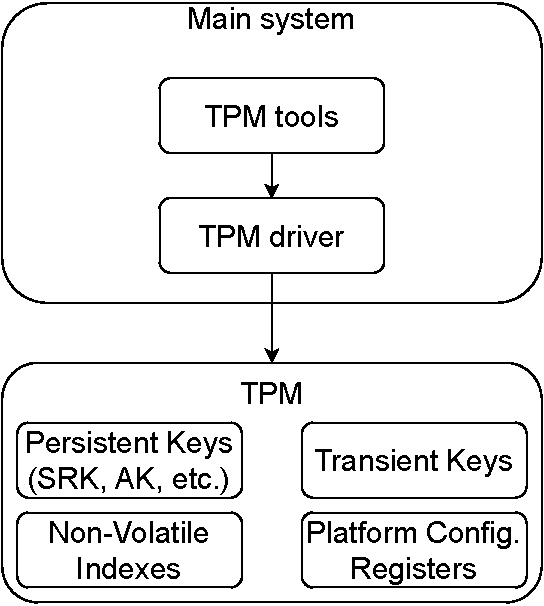
\includegraphics[width=0.5\textwidth]{ProtectingSshAuthenticationWithTpm20/img/tpm.pdf}
  \caption{Architecture of a system with a TPM}
  \label{fig:protectingsshauthenticationwithtpm20:tpmarchi}
\end{figure}

These features and many more (such as firmware upgrade, integration with
Intel SGX, etc.) have been well studied over the last decade.

For example several people used a TPM as a way to improve the security
of full-disk encryption by sealing a password used to decrypt the disk
(using the content of some PCRs and eventually a password called
\emph{TPM PIN code} to unseal the password). This is what Microsoft
implemented in BitLocker, which was presented at SSTIC in
2006~\cite{protectingsshauthenticationwithtpm20:sstic2006ourghanlian} and
in 2011~\cite{protectingsshauthenticationwithtpm20:sstic2011bordes}.
During the past two years, some people have been proposing to perform
something similar in \texttt{cryptsetup} for
Linux\footnote{\url{https://gitlab.com/cryptsetup/cryptsetup/-/merge_requests/51}}
and there was recent activity on this topic\footnote{\url{https://gitlab.com/cryptsetup/cryptsetup/-/merge_requests/98}}.

It is possible to restrict some operations on a TPM 2.0 using an
\emph{E/A policy} (Enhanced Authorization policy). This complex
mechanism was presented by Andreas Fuchs during Linux Security Europe
2020~\cite{protectingsshauthenticationwithtpm20:linseceu2020}.

Regarding the way TPM stores private keys, James Bottomley from IBM gave
a talk at the Kernel Recipes 2018
conference~\cite{protectingsshauthenticationwithtpm20:kernelrecipes2018}
and he repeatedly sent patches in order to store GnuPG keys in the
TPM\footnote{In 2018
  \url{https://lists.gnupg.org/pipermail/gnupg-devel/2018-January/033350.html}
  and in 2020
  \url{https://lists.gnupg.org/pipermail/gnupg-devel/2020-June/034621.html}}.
Such patches also help using SSH, as SSH can be configured to use GnuPG
keys for authentication. However at the time of writing, none of these
patches were accepted by GnuPG's developers, which is why this document
will not talk about GnuPG at all.

Regarding using a TPM to store SSH keys, several websites already
document the same commands as the one presented in the introduction (for
example
\url{https://medium.com/google-cloud/google-cloud-ssh-with-os-login-with-yubikey-opensc-pkcs11-and-trusted-platform-module-tpm-based-86fa22a30f8d},
\url{https://incenp.org/notes/2020/tpm-based-ssh-key.html} and
\url{https://linuxfr.org/news/utilisation-d-un-tpm-pour-l-authentification-ssh}).
But none of these websites dig into the details on how the key is stored
or how the SOPIN is actually implemented.

Even though many websites document how to use a TPM with SSH, only a few
people seem to actually use this. One of the reasons could be that
\texttt{tpm2-pkcs11} is a recent project which was not
properly packaged in Debian (and Ubuntu) before January 2021\footnote{\url{https://bugs.debian.org/cgi-bin/bugreport.cgi?bug=968310}}.
The author of this document helped fixing this and his contribution was
acknowledged by the package maintainer\footnote{\url{https://salsa.debian.org/debian/tpm2-pkcs11/-/commit/f76eb1d484dea1a38d0ad3fbdca779f84d1d9248}}.
Hopefully the future release of Debian 11 and Ubuntu 21.04 will provide
usable packages. A list of Linux distributions which package tpm2-pkcs11
can be found on Repology\footnote{\url{https://repology.org/project/tpm2-pkcs11/versions}}.

On the hardware level, several people took a look at TPM chips and their
communication channels. At Black Hat DC 2010, Christopher Tarnovsky
presented how he managed to dump the code running on an Infineon TPM
through advanced hardware
attacks~\cite{protectingsshauthenticationwithtpm20:bhdc2010}. Jeremy
Boone from NCC Group presented at CanSecWest 2018 how to build a device
which sits between some TPM and the CPU, called \emph{TPM
Genie}~\cite{protectingsshauthenticationwithtpm20:tpmgenie}. This device
enabled attackers to unseal the secrets used to encrypt a hard drive
encrypted with Microsoft's BitLocker. This attack was reproduced in 2020
by F-Secure~\cite{protectingsshauthenticationwithtpm20:fsecurebitlocker}.

On the cryptographic level, several vulnerabilities were discovered
throughout the years. In 2017, it was discovered that some TPM from
Infineon were generating RSA keys with a bias that enabled cracking them
in a reasonable amount of time (The Return of Coppersmith's Attack:
Practical Factorization of Widely Used RSA Moduli, ACM CCS
2017~\cite{protectingsshauthenticationwithtpm20:nemec2017return}). In
2019, it was discovered that the ECDSA implementations of some TPM from
Intel and STMicroelectronics were vulnerable to an attack which enabled
attackers to recover the private
key~\cite{protectingsshauthenticationwithtpm20:moghimi2020tpm}. These
attacks could compromise the SSH keys protected by the TPM. Nevertheless
these attacks do not mean that TPM and dedicated secure hardware are
worthless to store private keys: these attacks remain much more complex
to perform than stealing the private key stored in a file.

\section{Configuring a system to use a TPM 2.0 to secure SSH keys}

\subsection{Finding out whether a system has a TPM 2.0}

In order to study how a TPM 2.0 is used for SSH authentication, it is
necessary to have a software layer which implements a TPM 2.0 interface.
There are several ways of doing this.

But first, how is it possible to determine whether a TPM is available?
The usual tools that enable enumerating hardware components can help:

\begin{itemize}

\item
  The BIOS user interface/setup menu (available at boot time) might
  contain some configuration options related to the TPM, for example to
  enable it.
\item
  The filesystem might contain a device named
  \texttt{/dev/tpm0} and a non-empty directory
  \texttt{/sys/class/tpm}.
\item
  The kernel logs (command \texttt{dmesg}) might
  contain a line such as:
  \texttt{tpm\_tis NTC0702:00: 2.0 TPM (device-id 0xFC, rev-id 1)}.
\item
  Commands such as
  \texttt{fwupdmgr get-devices --show-all-devices}
  might give information about an existing TPM.
\item
  The author of this document also created a tool for Linux machines
  which represents in a graph the devices of a computer
  (\url{https://github.com/fishilico/home-files/blob/master/bin/graph-hw}).
  This tool was presented in a rump session at SSTIC
  2018~\cite{protectingsshauthenticationwithtpm20:sstic2018graphhw}.
\end{itemize}

When a TPM is present, a file could be present (since Linux 5.5) to
request the major version of the specification which is used
(listing~\ref{protectingsshauthenticationwithtpm20:sysclasstpmversionmajor}):

\begin{lstlisting}[language=sh, numbers=left, caption={Query the major version of the TPM used by the system, when using TPM 2.0}, label=protectingsshauthenticationwithtpm20:sysclasstpmversionmajor]
$ cat /sys/class/tpm/tpm0/tpm_version_major
2
\end{lstlisting}

Information such as the manufacturer of the TPM and product information
can be queried using \emph{TPM capabilities}. A command provided by
project \texttt{tpm2-tools} can be used to perform such
a query on a TPM 2.0
(listing~\ref{protectingsshauthenticationwithtpm20:tpm2getcappropsfixed}):

\begin{lstlisting}[language=sh, numbers=left, caption={Query all fixed properties from a TPM 2.0}, label=protectingsshauthenticationwithtpm20:tpm2getcappropsfixed]
$ tpm2_getcap --tcti device:/dev/tpmrm0 properties-fixed
TPM2_PT_FAMILY_INDICATOR:
  raw: 0x322E3000
  value: "2.0"
TPM2_PT_LEVEL:
  raw: 0
TPM2_PT_REVISION:
  value: 1.38
TPM2_PT_DAY_OF_YEAR:
  raw: 0x8
TPM2_PT_YEAR:
  raw: 0x7E2
TPM2_PT_MANUFACTURER:
  raw: 0x4E544300
  value: "NTC"
TPM2_PT_VENDOR_STRING_1:
  raw: 0x4E504354
  value: "NPCT"
TPM2_PT_VENDOR_STRING_2:
  raw: 0x37357800
  value: "75x"
TPM2_PT_VENDOR_STRING_3:
  raw: 0x2010024
  value: ""
TPM2_PT_VENDOR_STRING_4:
  raw: 0x726C7300
  value: "rls"
TPM2_PT_VENDOR_TPM_TYPE:
  raw: 0x0
TPM2_PT_FIRMWARE_VERSION_1:
  raw: 0x70002
TPM2_PT_FIRMWARE_VERSION_2:
  raw: 0x10000
\end{lstlisting}

Why is \texttt{/dev/tpmrm0} used in the command line?
When issuing commands to a TPM, it is recommended to use a \emph{TPM
Resource Manager}. This is because a TPM has a very limited capacity
which limits the number of cryptographic keys it can hold in memory. The
\emph{TPM Resource Manager} acts as a proxy to the TPM and enables using
any number of keys. It works by issuing
\texttt{ContextSave},
\texttt{ContextLoad} and
\texttt{FlushContext} commands to export, restore and
destroy data in its non-persistent memory. Doing so, the \emph{TPM
Resource Manager} gives the impression of using a TPM without any
capacity limit.

In practice, since Linux 4.12 (released in 2017) the kernel has been
implementing a \emph{TPM Resource Manager} which can be used through
device \texttt{/dev/tpmrm0}. Before, it was recommended
to use a user-space \emph{TPM Access Broker and Resource Manager Daemon}
(project \texttt{tpm2-abrmd}\footnote{\url{https://github.com/tpm2-software/tpm2-abrmd}})
instead of communicating with the device through
\texttt{/dev/tpm0}, but this recommendation does not
apply any more\footnote{cf.~\url{https://git.kernel.org/pub/scm/linux/kernel/git/torvalds/linux.git/commit/?id=fdc915f7f71939ad5a3dda3389b8d2d7a7c5ee66}
  for details}.

In order to query all the information which is available without
authentication from a TPM, the author of this document wrote a Python
script
(\url{https://github.com/fishilico/home-files/blob/master/bin/tpm-show}).

\subsection{Emulating a TPM 2.0}

If the system does not have a TPM 2.0 chip or if the user wants to
perform tests on a development TPM without breaking their real TPM, it
is possible to use a simulator. At the time of writing, there are mainly
two projects that can be used to launch a software TPM:

\begin{itemize}

\item
  \texttt{swtpm}\footnote{\url{https://github.com/stefanberger/swtpm}},
  which implements a front-end for
  \texttt{libtpms}\footnote{\url{https://github.com/stefanberger/libtpms}},
  a library which targets the integration of TPM functionality into
  hypervisors, primarily into QEMU.
\item
  \texttt{tpm\_server}\footnote{\url{https://github.com/kgoldman/ibmswtpm2}},
  which defines itself as an implementation of the TCG Trusted Platform
  Module 2.0 specification.
\end{itemize}

Both simulators are maintained by IBM, and the second one is based on
the TPM specification source code donated by Microsoft (according to its
\texttt{README}). In order to be able to use complex
commands with the simulators, it is required to use a TPM Resource
Manager such as \texttt{tpm2-abrmd}, which provides a
D-Bus service. Last but not least, each simulator uses a different
protocol to encapsulate TPM 2.0 commands. The protocol used by TPM tools
and libraries is configured through a mechanism called TCTI (TPM Command
Transmission Interface).

In short, launching a software TPM is quite complex but once all those
requirements are known, it is possible to document how it can be done.

Both simulators are packaged on several Linux distribution, including
Arch Linux. Readers who are interested in reproducing the instructions
of this section can start a container for example with
\texttt{podman run --rm -ti docker.io/library/archlinux}\footnote{Users
  more familiar with Docker can instead use:
  \texttt{sudo docker run --rm -ti docker.io/library/archlinux}}.

\begin{itemize}

\item
  To use \texttt{swtpm} (with TCTI library
  \texttt{/usr/lib/libtss2-tcti-swtpm.so},
  listing~\ref{protectingsshauthenticationwithtpm20:swtpmsetup}):
\end{itemize}

\begin{lstlisting}[language=sh, numbers=left, caption={Install and launch a TPM 2.0 simulator on Arch Linux, with \texttt{swtpm}}, label=protectingsshauthenticationwithtpm20:swtpmsetup]
pacman -Syu swtpm tpm2-abrmd tpm2-tools
swtpm socket --tpm2 --daemon \
    --server port=2321 --ctrl type=tcp,port=2322 \
    --flags not-need-init --tpmstate dir=/tmp \
    --log file=/tmp/swtpm.log,level=5
mkdir -p /run/dbus && dbus-daemon --system --fork
tpm2-abrmd --allow-root --tcti swtpm:host=127.0.0.1,port=2321 &
export TPM2TOOLS_TCTI=tabrmd:bus_type=system
\end{lstlisting}

\begin{itemize}

\item
  To use \texttt{tpm\_server} (with TCTI library
  \texttt{/usr/lib/libtss2-tcti-mssim.so}\footnote{MSSIM
    means \emph{Microsoft Simulator}. A few years ago, Microsoft
    published the source code of a TPM simulator and this code was
    modified to run on Linux in a program which became
    \texttt{tpm\_server}.
    \texttt{libtss2-tcti-mssim.so} implements the
    protocol used by this simulator.},
  listing~\ref{protectingsshauthenticationwithtpm20:tpmserversetup}):
\end{itemize}

\begin{lstlisting}[language=sh, numbers=left, caption={Install and launch a TPM 2.0 simulator on Arch Linux, with \texttt{tpm\_server}}, label=protectingsshauthenticationwithtpm20:tpmserversetup]
pacman -Syu ibm-sw-tpm2 tpm2-abrmd tpm2-tools
tpm_server -port 2321 > /tmp/tpm_server.log &
mkdir -p /run/dbus && dbus-daemon --system --fork
tpm2-abrmd --allow-root --tcti mssim:host=127.0.0.1,port=2321 &
export TPM2TOOLS_TCTI=tabrmd:bus_type=system
\end{lstlisting}

A third alternative consists in creating virtual devices very similar to
\texttt{/dev/tpm0} and
\texttt{/dev/tpmrm0} using a module called the
\emph{virtual TPM proxy} available since Linux 4.8
(listing~\ref{protectingsshauthenticationwithtpm20:swtpmvtpmsetup}):

\begin{lstlisting}[language=sh, numbers=left, caption={Install and launch a TPM 2.0 simulator on Arch Linux, with \texttt{swtpm} and the virtual TPM proxy}, label=protectingsshauthenticationwithtpm20:swtpmvtpmsetup]
pacman -Syu swtpm tpm2-tools
modprobe tpm_vtpm_proxy
swtpm chardev --tpm2 --vtpm-proxy --tpmstate dir=/var/lib/swtpm
\end{lstlisting}

In order to check that the software TPM launched by any of these
alternatives works fine, it is possible to query the TPM with
\texttt{tpm2\_getcap properties-fixed},
\texttt{tpm2\_pcrread}, etc.

The TPM Software Stack (TSS) includes a high-level interface called FAPI
(TSS 2.0 Feature Application Programming Interface). It is not possible
to directly use it with a software TPM because the default configuration
requires the presence of an Endorsement Key Certificate. In order to use
FAPI, a specific configuration file can be written to remove this
requirement
(listing~\ref{protectingsshauthenticationwithtpm20:tssfapiconfig}):

\begin{lstlisting}[language=sh, numbers=left, caption={Configure FAPI with a software TPM 2.0}, label=protectingsshauthenticationwithtpm20:tssfapiconfig]
echo > /etc/tpm2-tss/stpm_fapi_config.json \
    '{"profile_name": "P_ECCP256SHA256",' \
    '"profile_dir": "/etc/tpm2-tss/fapi-profiles/",' \
    '"user_dir": "~/.local/share/tpm2-tss/user/keystore",' \
    '"system_dir": "/var/lib/tpm2-tss/system/keystore",' \
    '"log_dir": "/run/tpm2_tss",' \
    '"tcti": "'"${TPM2TOOLS_TCTI}"'",' \
    '"system_pcrs": [],' \
    '"ek_cert_less": "yes"}'
export TSS2_FAPICONF=/etc/tpm2-tss/stpm_fapi_config.json
tss2_provision
\end{lstlisting}

The last command creates a SRK (Storage Root Key) usable by
\texttt{tpm2-pkcs11}, at the handle
\texttt{0x81000001}. This key is used to store private
keys and secrets in the TPM, in a way which guarantees some security
properties. Its public key can be read with
\texttt{tpm2\_readpublic -c 0x81000001}.

\section{tpm2-pkcs11 storage of the SSH key}

\subsection{Storage of the public key}

Back to \texttt{tpm2-pkcs11}: where is the private SSH
key stored and how is it decrypted?

The readers who are familiar with how TPMs are used in disk encryption
are likely to make the guess that the private key is simply
\emph{unsealed} from the TPM. That would mean that the key is known by
the software (the SSH client or one of its libraries) and that the TPM
is only used to store a passphrase for a private key file. However a TPM
can also directly load a private key and use it, without exposing it to
the software. Using this feature would strengthen the security of the
key storage. Therefore there appears to be a contradiction between some
intuition (that keys could be \emph{unsealed}) and the features of TPMs.
How is the private key processed?

The analysis of \texttt{tpm2-pkcs11} source code
reveals that private keys are indeed used by the TPM when performing
signature operations (using function
\texttt{Esys\_Sign} in
\url{https://github.com/tpm2-software/tpm2-pkcs11/blob/1.5.0/src/lib/tpm.c\#L1190}).

Nevertheless another file, \texttt{src/lib/utils.c}
contains calls to software implementation of AES-GCM, in function
\texttt{aes256\_gcm\_encrypt} and
\texttt{aes256\_gcm\_decrypt}. These functions appear
to be used to \emph{wrap} and \emph{unwrap} (which mean \emph{encrypt}
and \emph{decrypt}) some data named \texttt{objauth},
using the AES key which is unsealed from the TPM. In order to understand
what this \texttt{objauth} is, the persistent storage
of \texttt{tpm2-pkcs11} can be analyzed after the three
previous \texttt{tpm2\_ptool} commands from
listing~\ref{protectingsshauthenticationwithtpm20:ArchLinuxTpmCreate} are
issued.

This storage consists in a SQLite database which by default is created
in the home directory of the current user. It contains 5 tables when
using \texttt{tpm2-pkcs11} version 1.5.0
(listing~\ref{protectingsshauthenticationwithtpm20:sqltables}):

\begin{lstlisting}[language=sh, numbers=left, caption={Tables in \texttt{tpm2-pkcs11} database}, label=protectingsshauthenticationwithtpm20:sqltables]
$ sqlite3 "$HOME/.tpm2_pkcs11/tpm2_pkcs11.sqlite3"
sqlite> .tables
pobjects     schema       sealobjects  tobjects     tokens
\end{lstlisting}

These tables are used to link PKCS\#11 concepts to the TPM world.

In PKCS\#11, a slot may contain a token, which contains several objects
such as keys and certificates. Information about slots, tokens and
objects can be queried using command
\texttt{pkcs11-tool} from package
\texttt{opensc}
(listing~\ref{protectingsshauthenticationwithtpm20:pkcs11toolout}):

\begin{lstlisting}[numbers=left, caption={Output of \texttt{pkcs11-tool} on a system using a software TPM}, label=protectingsshauthenticationwithtpm20:pkcs11toolout]
$ pkcs11-tool --module /usr/lib/pkcs11/libtpm2_pkcs11.so \
    --show-info
Cryptoki version 2.40
Manufacturer     tpm2-software.github.io
Library          TPM2.0 Cryptoki (ver 0.0)
Using slot 0 with a present token (0x1)

$ pkcs11-tool --module /usr/lib/pkcs11/libtpm2_pkcs11.so \
    --list-token-slots
Available slots:
Slot 0 (0x1): ssh                             IBM
  token label        : ssh
  token manufacturer : IBM
  token model        : SW   TPM
  token flags        : login required, rng, token initialized,
PIN initialized
  hardware version   : 1.50
  firmware version   : 23.25
  serial num         : 0000000000000000
  pin min/max        : 0/128
Slot 1 (0x2):                                 IBM
  token state:   uninitialized

$ pkcs11-tool --module /usr/lib/pkcs11/libtpm2_pkcs11.so \
    --list-objects
Using slot 0 with a present token (0x1)
Public Key Object; EC  EC_POINT 256 bits
  EC_POINT:   0441043eef05ada9dc42f69ffca066adfc374ec94aaba63bfa
9383c2a563d847f31ac250702adc8e1081d1b633a1e1d6278b4613ba20cf5fd8
af0b8c3c8b4a765b9387
  EC_PARAMS:  06082a8648ce3d030107
  label:
  ID:         35386461383061353363366536643935
  Usage:      encrypt, verify
  Access:     local
\end{lstlisting}

These commands did not interact with the TPM, even though the content of
the generated public key was displayed\footnote{This was observed by
  recording the system calls issued by the commands using
  \texttt{strace}. The commands did not interact with
  any device related to TPM.}. This information is indeed stored in the
SQLite database. More precisely, the \texttt{tobjects}
table contains information about \emph{transient objects}, including all
their associated PKCS\#11 attributes. These attributes can be decoded
using constants defined in \texttt{tpm2-pkcs11}'s
code\footnote{\url{https://github.com/tpm2-software/tpm2-pkcs11/blob/1.5.0/tools/tpm2_pkcs11/pkcs11t.py\#L39-L97}}
and for example the elliptic curve public key is stored in attribute
\texttt{CKA\_EC\_POINT = 0x181}.

\texttt{tpm2-pkcs11} defines three \emph{vendor
attributes}: \texttt{CKA\_TPM2\_OBJAUTH\_ENC},
\texttt{CKA\_TPM2\_PUB\_BLOB} and
\texttt{CKA\_TPM2\_PRIV\_BLOB}. In the SQLite database
used for tests, there are 2 objects:

\begin{itemize}

\item
  One with attribute 0 set to 3, which means that its
  \texttt{CKA\_CLASS} is
  \texttt{CKO\_PRIVATE\_KEY}: it is a private key. This
  object also contains the three \emph{vendor attributes} of
  \texttt{tpm2-pkcs11}.
\item
  The other one with attribute 0 set to 2, which means that its
  \texttt{CKA\_CLASS} is
  \texttt{CKO\_PUBLIC\_KEY}: it is a public key. This
  object only has \texttt{CKA\_TPM2\_PUB\_BLOB} as
  \emph{vendor attribute}.
\end{itemize}

For both objects, attribute
\texttt{CKA\_TPM2\_PUB\_BLOB} contains
hexadecimal-encoded data which includes the elliptic curve public key.
In fact, this attribute stores data encoded according to a structure
which is defined in TPM 2.0 specification as
\texttt{TPM2B\_PUBLIC}
(listing~\ref{protectingsshauthenticationwithtpm20:structtpm2bpublic},
from
\url{https://github.com/stefanberger/libtpms/blob/v0.7.5/src/tpm2/TpmTypes.h\#L1682-L1695}):

\begin{lstlisting}[language=C, numbers=left, caption={Structures \texttt{TPMT\_PUBLIC} and \texttt{TPM2B\_PUBLIC} from TPM 2.0 specification}, label=protectingsshauthenticationwithtpm20:structtpm2bpublic]
typedef struct {
    TPMI_ALG_PUBLIC         type;
    TPMI_ALG_HASH           nameAlg;
    TPMA_OBJECT             objectAttributes;
    TPM2B_DIGEST            authPolicy;
    TPMU_PUBLIC_PARMS       parameters;
    TPMU_PUBLIC_ID          unique;
} TPMT_PUBLIC;
typedef struct {
    UINT16                  size;
    TPMT_PUBLIC             publicArea;
} TPM2B_PUBLIC;
\end{lstlisting}

For example, when the content of attribute
\texttt{CKA\_TPM2\_PUB\_BLOB} is
(listing~\ref{protectingsshauthenticationwithtpm20:pubblobexampleraw}):

\begin{lstlisting}[numbers=left, caption={Example of generated public key blob}, label=protectingsshauthenticationwithtpm20:pubblobexampleraw]
00560023000b000600720000001000100003001000203eef05ada9dc42f69ffc
a066adfc374ec94aaba63bfa9383c2a563d847f31ac2002050702adc8e1081d1
b633a1e1d6278b4613ba20cf5fd8af0b8c3c8b4a765b9387
\end{lstlisting}

This content can be decoded as
(listing~\ref{protectingsshauthenticationwithtpm20:pubblobexampledec}):

\begin{lstlisting}[language=C, numbers=left, caption={Deserialization of an example of generated public key blob}, label=protectingsshauthenticationwithtpm20:pubblobexampledec]
struct TPM2B_PUBLIC {
  size = 0x0056,
  publicArea = {
    type = 0x0023, // = TPM_ALG_ECC
    nameAlg = 0x000b, // = TPM_ALG_SHA256
    objectAttributes = 0x00060072,
    authPolicy = { size = 0x0000 },
    parameters.eccDetail = {
      symmetric = 0x0010, // = TPM_ALG_NULL
      scheme = 0x0010, // = TPM_ALG_NULL
      curveID = 0x0003, // = TPM_ECC_NIST_P256
      kdf = 0x0010 // = TPM_ALG_NULL
    },
    unique.ecc = {
      x = {
        size = 0x0020,
        bytes = "3eef05ada9dc42f69ffca066adfc374e"
                "c94aaba63bfa9383c2a563d847f31ac2"
      },
      y = {
        size = 0x0020,
        bytes = "50702adc8e1081d1b633a1e1d6278b46"
                "13ba20cf5fd8af0b8c3c8b4a765b9387"
      }
    }
  }
}
\end{lstlisting}

So attribute \texttt{CKA\_TPM2\_PUB\_BLOB} directly
consists in the public key generated with
\texttt{tpm2\_ptool addkey}, serialized for the TPM.
Does attribute \texttt{CKA\_TPM2\_PRIV\_BLOB} directly
contains the associated private key? The answer should of course be
negative, and some further analysis was conducted in order to understand
why something related to the private key is stored in the database.

\subsection{Storage of the private key}

From a functional point of view, a TPM only has a limited amount of
persistent memory but it is able to use many keys. This is made possible
because the private keys are stored outside of the TPM and are encrypted
with a secret which never leaves the TPM. When a private key is used for
example to perform some signing operations, the key first needs to be
loaded into the TPM. The TPM decrypts the private key before loading it.

In practice, the encrypted private key is serialized with a structure
defined in TPM 2.0 specification as
\texttt{TPM2B\_PRIVATE}, which only states ``a size and
some bytes''. When using the TPM simulator
\texttt{swtpm}, it is possible to retrieve the
encryption key and to decrypt the private key.

In the tests, the content of attribute
\texttt{CKA\_TPM2\_PRIV\_BLOB} is
(listing~\ref{protectingsshauthenticationwithtpm20:privblobexampleraw}):

\begin{lstlisting}[numbers=left, caption={Example of generated private key blob}, label=protectingsshauthenticationwithtpm20:privblobexampleraw]
007e002093b2e33a7ff39879229e35afeb86ec61bca0aaee057c0d56bee354bc
41cc01f50010627e422444e01671fe6b2e3a771634d64d64599bc3129fb57f10
2bb89244e6d7c6c029a9a53b27bddbb0ba5b5fa0497c3286364b50fce3757615
c895de4fce053c4793a4b39b35007fb7d2a29557b9b318b15ecbd4f7c70908a8
\end{lstlisting}

This can be decoded as
(listing~\ref{protectingsshauthenticationwithtpm20:privblobexampledec}):

\begin{lstlisting}[language=C, numbers=left, caption={Deserialization of an example of generated private key blob}, label=protectingsshauthenticationwithtpm20:privblobexampledec]
struct TPM2B_PRIVATE {
  size = 0x007e,
  buffer = {
    integrity = {
      size = 0x0020,
      bytes = "93b2e33a7ff39879229e35afeb86ec61"
              "bca0aaee057c0d56bee354bc41cc01f5"
    },
    iv = {
      size = 0x0010,
      bytes = "627e422444e01671fe6b2e3a771634d6"
    },
    encrypted =
      "4d64599bc3129fb57f102bb89244e6d7c6c029a9a53b27bd"
      "dbb0ba5b5fa0497c3286364b50fce3757615c895de4fce05"
      "3c4793a4b39b35007fb7d2a29557b9b318b15ecbd4f7c709"
      "08a8"
  }
}
\end{lstlisting}

In order to decrypt the data, the persistent storage of the software TPM
needs to be analyzed. This storage is located in a file named
\texttt{tpm2-00.permall} in the directory specified by
option \texttt{--tpmstate} when launching
\texttt{swtpm}. This file contains the public and
sensitive structures (\texttt{TPMT\_PUBLIC} and
\texttt{TPMT\_SENSITIVE} in TPM specification) related
to the SRK (Storage Root Key) used by
\texttt{tpm2-pkcs11} and defined by handle
\texttt{0x81000000}. A sensitive structure contains the
following fields
(listing~\ref{protectingsshauthenticationwithtpm20:structtpmtsensitive}):

\begin{lstlisting}[language=C, numbers=left, caption={Structure \texttt{TPMT\_SENSITIVE} from TPM 2.0 specification}, label=protectingsshauthenticationwithtpm20:structtpmtsensitive]
typedef struct {
    TPMI_ALG_PUBLIC             sensitiveType;
    TPM2B_AUTH                  authValue;
    TPM2B_DIGEST                seedValue;
    TPMU_SENSITIVE_COMPOSITE    sensitive;
} TPMT_SENSITIVE;
\end{lstlisting}

In the file used in the tests, the content of
\texttt{seedValue} is in hexadecimal
(listing~\ref{protectingsshauthenticationwithtpm20:seedvalue}):

\begin{lstlisting}[numbers=left, caption={\texttt{seedValue} of the SRK used in tests}, label=protectingsshauthenticationwithtpm20:seedvalue]
07f5b590a03d66e2225274698323ccfe59a7356e9cc14436091fe9d49b3e577c
\end{lstlisting}

Using this value, it is possible to derive a HMAC key and an AES key, to
verify the integrity tag and to decrypt the data.

Here is a Python 3.8 session showing how to compute those values
(listing~\ref{protectingsshauthenticationwithtpm20:seedderivation}):

\begin{lstlisting}[language=Python, numbers=left, caption={Python session which decrypts a private key blob using the \texttt{seedValue} of the SRK and the \emph{public name} associated with the key}, label=protectingsshauthenticationwithtpm20:seedderivation]
>>> import hashlib, hmac

>>> pub_blob = bytes.fromhex("""
... 00560023000b000600720000001000100003001000203eef05ada9dc42f69ffc
... a066adfc374ec94aaba63bfa9383c2a563d847f31ac2002050702adc8e1081d1
... b633a1e1d6278b4613ba20cf5fd8af0b8c3c8b4a765b9387
... """)
>>> priv_blob = bytes.fromhex("""
... 007e002093b2e33a7ff39879229e35afeb86ec61bca0aaee057c0d56bee354bc
... 41cc01f50010627e422444e01671fe6b2e3a771634d64d64599bc3129fb57f10
... 2bb89244e6d7c6c029a9a53b27bddbb0ba5b5fa0497c3286364b50fce3757615
... c895de4fce053c4793a4b39b35007fb7d2a29557b9b318b15ecbd4f7c70908a8
... """)
>>> srk_seed = bytes.fromhex("""
... 07f5b590a03d66e2225274698323ccfe59a7356e9cc14436091fe9d49b3e577c
... """)

# Compute the public name, prefixed by TPM_ALG_SHA256 = 0x000b
>>> pub_name = b'\x00\x0b' + hashlib.sha256(pub_blob[2:]).digest()
>>> pub_name.hex()
'000bcac322c64b1a31d7806bc84570090949f898cea8c2c9a258761659dfb1de'
'713d'

# Compute HMAC key with KDFa
>>> hashstate = hmac.new(srk_seed, None, "sha256")
>>> hashstate.update(int.to_bytes(1, 4, "big"))  # counter
>>> hashstate.update(b'INTEGRITY\0')  # label
>>> hashstate.update(int.to_bytes(256, 4, "big"))  # sizeInBits
>>> hmac_key = hashstate.digest()
>>> hmac_key.hex()
'7f861102ab2854de213e6ffa9ae2a2521c73abf49b697618736d85615d27389b'

# Compute the integrity tag
>>> hashstate = hmac.new(hmac_key, None, "sha256")
>>> hashstate.update(priv_blob[0x24:])
>>> hashstate.update(pub_name)
>>> computed_integrity = hashstate.digest()
>>> computed_integrity.hex()
'93b2e33a7ff39879229e35afeb86ec61bca0aaee057c0d56bee354bc41cc01f5'

# Check the integrity
>>> computed_integrity == priv_blob[4:0x24]
True

# Compute the AES key with KDFa
>>> hashstate = hmac.new(srk_seed, None, "sha256")
>>> hashstate.update(int.to_bytes(1, 4, "big"))  # counter
>>> hashstate.update(b'STORAGE\0')  # label
>>> hashstate.update(pub_name)  # contextU = name
>>> hashstate.update(int.to_bytes(128, 4, "big"))  # sizeInBits
>>> aes_key = hashstate.digest()[:16]
>>> aes_key.hex()
'9052599459c554ee409ffdba6311b2ce'

# Decrypt private blob using library cryptography.io
>>> from cryptography.hazmat.primitives.ciphers import \
...   Cipher, algorithms, modes
>>> from cryptography.hazmat.backends import default_backend
>>> iv = priv_blob[0x26:0x36]
>>> cipher = Cipher(algorithms.AES(aes_key), modes.CFB(iv),
...   backend=default_backend())
>>> sensitive = cipher.decryptor().update(priv_blob[0x36:])
>>> sensitive.hex()
'0048002300203036343132623637616663383763303765626132366334653031'
'61653662353000000020e136a90d627a7b2ea404ed671a7717cb04b13f54f9df'
'478ff54ced6fd3275048'
\end{lstlisting}

The decrypted sensitive structure can be decoded as
(listing~\ref{protectingsshauthenticationwithtpm20:sensitiveblobexampledec}):

\begin{lstlisting}[language=C, numbers=left, caption={Deserialization of the decryption of a generated private key blob}, label=protectingsshauthenticationwithtpm20:sensitiveblobexampledec]
struct TPM2B_SENSITIVE {
  size = 0x0048,
  sensitiveArea = {
    sensitiveType = 0x0023, // = TPM_ALG_ECC
    authValue = {
      size = 0x0020,
      buffer = "30363431326236376166633837633037"
               "65626132366334653031616536623530"
    },
    seedValue = { size = 0x0000 },
    sensitive.ecc = {
      size = 0x0020,
      buffer = "e136a90d627a7b2ea404ed671a7717cb"
               "04b13f54f9df478ff54ced6fd3275048"
    }
  }
}
\end{lstlisting}

The last buffer, \texttt{sensitive.ecc}, contains the
private key associated with the elliptic curve public key
(listing~\ref{protectingsshauthenticationwithtpm20:eccderiv}):

\begin{lstlisting}[language=Python, numbers=left, caption={Python session which computes the public key associated with the recovered private key}, label=protectingsshauthenticationwithtpm20:eccderiv]
>>> from cryptography.hazmat.primitives.asymmetric import ec
>>> from cryptography.hazmat.backends import default_backend
>>> sensitive_ecc_buffer = bytes.fromhex(
...  "e136a90d627a7b2ea404ed671a7717cb"
...  "04b13f54f9df478ff54ced6fd3275048")
>>> privkey = ec.derive_private_key(
...  int.from_bytes(sensitive_ecc_buffer, "big"),
...  curve=ec.SECP256R1(),
...  backend=default_backend())
>>> pubkey = privkey.public_key()
>>> hex(pubkey.public_numbers().x)
'0x3eef05ada9dc42f69ffca066adfc374ec94aaba63bfa9383c2a563d847f31ac2'
>>> hex(pubkey.public_numbers().y)
'0x50702adc8e1081d1b633a1e1d6278b4613ba20cf5fd8af0b8c3c8b4a765b9387'
\end{lstlisting}

This confirms that \texttt{tpm2-pkcs11}'s database
contains an encrypted version of the private key, stored in attribute
\texttt{CKA\_TPM2\_PRIV\_BLOB} of the PKCS\#11 object
associated with the private key. This attribute is encrypted using the
\texttt{seedValue} of the used SRK, which is a secret
supposed to never leave the TPM. Therefore this analysis also confirms
that only the TPM itself can decrypt this attribute.

Now, there is something strange with this analysis: neither the user PIN
nor the SOPIN were used to decrypt the private key. And indeed they are
not needed to load the key
(listing~\ref{protectingsshauthenticationwithtpm20:tpm2loadpriv}):

\begin{lstlisting}[language=sh, numbers=left, caption={Loading private key blob and public key blob in the TPM}, label=protectingsshauthenticationwithtpm20:tpm2loadpriv]
# Load the key with file "pub_blob" containing the content
# of CKA_TPM2_PUB_BLOB and "priv_blob" the content of
# CKA_TPM2_PRIV_BLOB
$ tpm2_load -c /tmp/context -C 0x81000000 \
    -u pub_blob -r priv_blob
name: 000bcac322c64b1a31d7806bc84570090949f898cea8c2c9a2587
61659dfb1de713d
\end{lstlisting}

But using this key does not directly work to sign data
(listing~\ref{protectingsshauthenticationwithtpm20:tpm2signfail}):

\begin{lstlisting}[language=sh, numbers=left, caption={Trying to use the key to sign a message produces errors}, label=protectingsshauthenticationwithtpm20:tpm2signfail]
$ echo hello | tpm2_sign -c /tmp/context \
    -g sha256 -s ecdsa -o signature.out
WARNING:esys:src/tss2-esys/api/Esys_Sign.c:311:Esys_Sign_Finish()
Received TPM Error
ERROR:esys:src/tss2-esys/api/Esys_Sign.c:105:Esys_Sign()
Esys Finish ErrorCode (0x0000098e)
ERROR: Eys_Sign(0x98E) - tpm:session(1):the authorization
HMAC check failed and DA counter incremented
ERROR: Unable to run tpm2_sign
\end{lstlisting}

The error suggests an authentication failure, with the DA counter
(Dictionary Attack) of the TPM being incremented\footnote{The Dictionary
  Attack counter is a mechanism which prevents brute-force attacks on
  TPM. After some number of authentication failures, the TPM becomes
  locked and rejects any further authentication try.}.

In the decrypted sensitive structure associated with the private key
(listing~\ref{protectingsshauthenticationwithtpm20:sensitiveblobexampledec}),
the \texttt{authValue} contains 32 bytes which are
represented in hexadecimal. In practice these bytes consist in 32
hexadecimal characters:
\texttt{06412b67afc87c07eba26c4e01ae6b50}. This value
can be directly used with command \texttt{tpm2\_sign}
to sign a message without any error
(listing~\ref{protectingsshauthenticationwithtpm20:tpm2signauth}):

\begin{lstlisting}[language=sh, numbers=left, caption={Trying to use the key to sign a message with the \texttt{authValue} (parameter \texttt{-p} succeeds}, label=protectingsshauthenticationwithtpm20:tpm2signauth]
$ echo hello | tpm2_sign -c /tmp/context \
    -g sha256 -s ecdsa -o signature \
    -p 06412b67afc87c07eba26c4e01ae6b50
$ xxd -p -c32 signature
0018000b00201f076fa127366b9d9cc36155652751545115e4ce35749ed75638
7e68f058d35d00203bd83b9086a7876948fcc4728c4141b30a0fe94cada03147
76052933888802a8

# Verifying the signature does not require the authValue
$ echo hello > msg
$ tpm2_verifysignature -c /tmp/context -s signature -m msg
\end{lstlisting}

Therefore the private key generated with
\texttt{tpm2\_ptool addkey} is protected by an
authorization value. In the presented tests, this authorization value
was retrieved by decrypting the private blob exported by the TPM. Doing
so was possible only because a software TPM was used and the decryption
key could be retrieved. With a hardware TPM, this should not be
possible. There should be another way to retrieve it,
\texttt{tpm2-pkcs11} needs to be able to use the key.

\section{Linking the PIN of the PKCS\#11 token with the authorization
value of the key}

\subsection{Unsealing a wrapping key from the PIN or the SOPIN}

The previous section presented that the private SSH key generated with
\texttt{tpm2\_ptool addkey} was stored in a PKCS\#11
attribute (named \texttt{CKA\_TPM2\_PRIV\_BLOB}) in
table \texttt{tobjects} of
\texttt{tpm2-pkcs11}'s SQLite database. This private
key was (of course) encrypted by the TPM and in order to use it, the
software has to provide an authorization value to the TPM.

Taking a step back, the PIN and the SOPIN should be linked to this
authorization value: both are some kind of secret that the user is
required to enter in order to use the key. But the PIN and the SOPIN are
two independent secrets: the PIN can be used without the SOPIN when
using the key and if the PIN is forgotten, the SOPIN can be used to
reset the PIN.

In order to help understanding how this works,
\texttt{tpm2-pkcs11} provides a command,
\texttt{tpm2\_ptool verify}. This command checks the
PIN or the SOPIN (or both) and displays some hexadecimal values such as
\texttt{seal-auth} and
\texttt{wrappingkey}. None of these values match the
authorization value which was found in the previous section. While
investigating why, the author of this document found a bug in the Python
code of the tool (a variable was not initialized when some options were
provided) and fixed it\footnote{\url{https://github.com/tpm2-software/tpm2-pkcs11/pull/635}}.
But this fix did not change the fact that
\texttt{tpm2\_ptool verify} did not show the
authorization value, so it was necessary to dig a little bit more.

The SQLite database used by \texttt{tpm2-pkcs11}
includes a table named \texttt{sealobjects} which is
used to store information for the PIN and SOPIN
(listing~\ref{protectingsshauthenticationwithtpm20:sqlsealobjects}):

\begin{lstlisting}[language=sh, numbers=left, caption={Content of \texttt{sealobjects} database in \texttt{tpm2-pkcs11} database}, label=protectingsshauthenticationwithtpm20:sqlsealobjects]
$ sqlite3 "$HOME/.tpm2_pkcs11/tpm2_pkcs11.sqlite3"
sqlite> .dump sealobjects
PRAGMA foreign_keys=OFF;
BEGIN TRANSACTION;
CREATE TABLE sealobjects(
    id INTEGER PRIMARY KEY,
    tokid INTEGER NOT NULL,
    userpub BLOB,
    userpriv BLOB,
    userauthsalt TEXT,
    sopub BLOB NOT NULL,
    sopriv BLOB NOT NULL,
    soauthsalt TEXT NOT NULL,
    FOREIGN KEY (tokid) REFERENCES tokens(id) ON DELETE CASCADE
);
INSERT INTO sealobjects VALUES(1,1,
X'002e0008000b00000052000000100020b0c383025b2418e95f530707ba7f28
a29b4bf55d65f004c8365c68400ae3cc60',
X'00be0020835e6bbbc97ff76714b0b9cc7352d823cc250741ecb2817c7ad28b
44d958cfc3001084d9eb99781ba29b9e2dfc601ae5bec4fdcbce5055be161244
5f67e390b54328ae4b47f126746393ba7dcc9dc7b93b766f761473d68d581dfd
aed3d6a365ce9bb90d7d2cb1118363f4416b1770dbdbfa726b480c760f113b69
6556b064ebce1b05ac8d80511c83f753f5aeb342257b5b561ba746dc2ccafd0f
5e2824c3f7838c235115b75d1665c7938a0a50999990a1399194ee9aa0eb03f8
36',
X'37323832653632346561643164656331613761653539386234363065656336
6335663736633730646562623234663335376664613531313437653937333365
34',
X'002e0008000b00000052000000100020df41af69b73d88f829c60fe0e27687
62f43be4e831cc0a5d0af5508b1752cecf',
X'00be002013579162beec11b58bbd5ac9d4db3b1f2de8a70f276f75b1925111
06ad76ff100010f937771c1214098ad9a19d49a211757f2d1f9d48195624e87c
526ad8ccb229479a474aa7ba3b010058ad64f33560aad3529c6e4a1c10092304
5cddd249fec9d565bb037712ffc267c9837d8ca561f6d720d84ddf019dc8fe45
c059e34dc20b258f0f2c959aca09cb580eadecc1f3fdae44587d51f9028f50b4
6b9e7007538751508d49f52a21426357c72671f4915562ab9cd7b18cb28a77ac
6c',
X'62633235333163643434633466333166313239663437613738636664333834
6563636538363533343662633936623263633239623135306262306462646362
38');
\end{lstlisting}

Columns \texttt{userpub} and
\texttt{sopub} both store a
\texttt{TPM2B\_PUBLIC} structure
(listing~\ref{protectingsshauthenticationwithtpm20:userpubblobexampledec}):

\begin{lstlisting}[language=C, numbers=left, caption={Extract of the deserialization of the content of \texttt{userpub} and \texttt{sopub} columns}, label=protectingsshauthenticationwithtpm20:userpubblobexampledec]
struct TPM2B_PUBLIC {
  size = 0x002e,
  publicArea = {
    type = 0x0008, // = TPM_ALG_KEYEDHASH
    nameAlg = 0x000b, // = TPM_ALG_SHA256
    objectAttributes = 0x00000052,
    authPolicy = { size = 0x0000 },
    parameters.keyedHashDetail = {
      scheme = 0x0010 // = TPM_ALG_NULL
    },
    unique.keyedHash = {
      size = 0x0020,
      bytes = "..."
    }
  }
}
\end{lstlisting}

This structure is a \emph{Keyed Hash} object, which is in theory a way
to store a secret key to perform a HMAC-based authentication. In
practice, this object is used here to store a \emph{sealed} secret (it
cannot be used as a HMAC authentication because
\texttt{parameters.keyedHashDetail.scheme} is
\texttt{TPM\_ALG\_NULL}), in the private parts which
are in columns \texttt{userpriv} and
\texttt{sopriv}. In order to \emph{unseal} the secret,
the public and private parts need to be loaded in the TPM, and then
\texttt{tpm2\_unseal} can be used with an authorization
value derived from the PIN (when using
\texttt{userpub}/\texttt{userpriv}) or
the SOPIN (when using
\texttt{sopub}/\texttt{sopriv}). This
authorization value only consists in the SHA256 digest of the PIN
concatenated with the value in column
\texttt{userauthsalt} or
\texttt{soauthsalt}, truncated to 16 bytes
(listings~\ref{protectingsshauthenticationwithtpm20:usersealauthderiv}
and~\ref{protectingsshauthenticationwithtpm20:usersealauthtest}):

\begin{lstlisting}[language=Python, numbers=left, caption={Python session which computes the authorization value of the \texttt{userpub} field, from the user PIN and \texttt{userauthsalt}}, label=protectingsshauthenticationwithtpm20:usersealauthderiv]
>>> from hashlib import sha256
>>> userpin = b"XXXX"
>>> userauthsalt = bytes.fromhex("""
... 3732383265363234656164316465633161376165353938623436306565633663
... 3566373663373064656262323466333537666461353131343765393733336534
... """)
>>> usersealauth = sha256(userpin + userauthsalt).digest()[:16]
>>> usersealauth.hex()
'c3402eac59ae76a86317d9b34811ca3d'
\end{lstlisting}

\begin{lstlisting}[language=sh, numbers=left, caption={Using the derived authorization value to unseal the \texttt{userpriv} field}, label=protectingsshauthenticationwithtpm20:usersealauthtest]
$ tpm2_load -c /tmp/context -C 0x81000000 \
    -u userpub -r userpriv
$ tpm2_unseal -c /tmp/context -p c3402eac59ae76a86317d9b34811ca3d
9d7854e46e3e8816070697c9770fbc2ed4297dea669bebbe2c22a52421df63cd
\end{lstlisting}

If the authorization value is wrong or missing,
\texttt{tpm2\_unseal} fails and returns the error
message ``the authorization HMAC check failed and DA counter
incremented''. This indicates that the \emph{sealed} secret is protected
by the TPM's Dictionary Attack counter which prevents brute-force
attacks.

Moreover, repeating the commands with the SOPIN and its associated
fields leads to the same secret being \emph{unsealed}. This secret
(encoded in hexadecimal) is also displayed by command
\texttt{tpm2\_ptool verify} using the name
\emph{wrappingkey}.

\subsection{Decrypting an authorization value from the wrapping key}

The previous sections presented that:

\begin{itemize}

\item
  the SSH key generated with
  \texttt{tpm2\_ptool addkey} was protected by an
  authorization value,
\item
  and the PIN and or SOPIN of a \emph{token} enabled \emph{unsealing} a
  \emph{wrapping key} which was not this authorization value.
\end{itemize}

Something is missing to establish a link between \emph{wrapping key} and
the authorization value. Studying how
\texttt{tpm2-pkcs11} works enabled bridging the gap:
the \emph{wrapping key} is an AES key which is used to encrypt the
authorization value using AES-GCM. The encrypted value and the
parameters of the GCM mode (a nonce and a tag) are stored in attribute
\texttt{CKA\_TPM2\_OBJAUTH\_ENC} of each private key,
in table \texttt{tobjects} of the SQLite database.

In the tests, this attribute contains
(listing~\ref{protectingsshauthenticationwithtpm20:objauthencraw}):

\begin{lstlisting}[numbers=left, caption={Attribute \texttt{CKA\_TPM2\_OBJAUTH\_ENC} of the generated SSH key}, label=protectingsshauthenticationwithtpm20:objauthencraw]
3638333330346435336435306134376466356666383530333a33313632626439
366639313431656463323265613836663664666137396466653a663036323866
3066353661373637656261316361393631376239396234613162643561653666
3662653863323664623966383932373765666531393137343234
\end{lstlisting}

Here is a Python 3.8 session showing how to decode this data, using the
wrapping key unsealed in
listing~\ref{protectingsshauthenticationwithtpm20:usersealauthtest}
(listing~\ref{protectingsshauthenticationwithtpm20:authvalderiv}):

\begin{lstlisting}[language=Python, numbers=left, caption={Python session which computes the authorization value of a key from the wrapping key}, label=protectingsshauthenticationwithtpm20:authvalderiv]
>>> from cryptography.hazmat.primitives.ciphers.aead import AESGCM
>>> objauth_enc_unhex = bytes.fromhex("""
... 3638333330346435336435306134376466356666383530333a33313632626439
... 366639313431656463323265613836663664666137396466653a663036323866
... 3066353661373637656261316361393631376239396234613162643561653666
... 3662653863323664623966383932373765666531393137343234
... """)
>>> fields = objauth_enc_unhex.decode("ascii").split(":")
>>> nonce, tag, ciphertext = map(bytes.fromhex, fields)

>>> wrappingkey = bytes.fromhex("""
... 9d7854e46e3e8816070697c9770fbc2ed4297dea669bebbe2c22a52421df63cd
... """)
>>> aesgcm = AESGCM(wrappingkey)
>>> authval = aesgcm.decrypt(nonce, ciphertext + tag, b'')
>>> authval
b'06412b67afc87c07eba26c4e01ae6b50'
\end{lstlisting}

This last value is indeed the authorization value embedded in the
sensitive structure of the private key which was generated
(listing~\ref{protectingsshauthenticationwithtpm20:sensitiveblobexampledec}).

In short, the PIN and the SOPIN are used by
\texttt{tpm2-pkcs11} to \emph{unseal} an AES key which
is used to decrypt (without using the TPM) the authorization value which
is necessary to use keys, for example to sign data or to perform SSH
authentication.

\section{Conclusion}

When using \texttt{tpm2-pkcs11} 1.5.0 to generate and
handle SSH keys with a TPM 2.0, the software never sees the private
keys. They are exported by the TPM in \emph{private blobs} that
\texttt{tpm2-pkcs11} stores in a database. To use these
keys, an authorization value needs to be provided to the TPM and
\texttt{tpm2-pkcs11} stores an encrypted copy of this
value which relies on a complex derivation scheme.

This enables to answer the questions which were asked in the
introduction:

\begin{itemize}

\item
  Is stealing the SQLite database enough to impersonate the user? No, as
  the keys it contains are encrypted using the TPM's SRK.
\item
  Is there any software (which could be compromised) that sees the
  private key when the user uses it to connect to a server? No.
\item
  How is the TPM actually used to authenticate the user? The key is
  loaded into the TPM, the software computes an authorization value
  using the PIN or the SOPIN. It then requests the TPM to use the key to
  perform a signature operation used in the authentication protocol.
\end{itemize}

Moreover, even though this article focused on SSH, the software stack
provides a compatibility layer with many other protocols through a
PKCS\#11 interface. For example this enables transposing the questions
and their answers to VPN software (Virtual Private Network), TLS stacks
(Transport Layer Security), etc.

Knowing how \texttt{tpm2-pkcs11} works in detail would
enable assessing its security. This could be done in some future work.

\bibliography{ProtectingSshAuthenticationWithTpm20/biblio}
